\documentclass{article}
\usepackage[margin=1in]{geometry}
\usepackage{microtype}
\usepackage{setspace}
\usepackage{amsmath}
\usepackage{parskip}
\usepackage{amssymb}
\usepackage{graphicx}

\graphicspath{{../public/}}

\parskip=4ex
\date{}
\author{}

\title{4.4 Coordinate Systems}

\begin{document}
  \maketitle
  \textbf{Theorem 3.8 The Unique Representation Theorem}\\
  Let $ \mathcal{B}=\{ b_1,...,b_n \} $ be a basis for a vector space $ V $. Then for each $ x $ in $ V $, there exists a unique set of scalars $ c_1,...,c_n $ such that
  \[
    x=c_1b_1+...+c_nb_n
  \]

  \textbf{Definition}\\
  Suppouse $ \mathcal{B}=\{ b_1,...,b_n \} $ is a basis for a vector space $ V $ and $ x $ is in $ V $. The coordinates of $ x $ relative to the basis $ \mathcal{B} $ (or the $ \mathcal{B} $ coordinates of $ x$) are the weights $ c_1,...,c_n $ such that $ x=c_1b_1+...+c_nb_n $. 
  
  If $ c_1,...,c_n $ are the $ \mathcal{B} $ coordinates of $ x $, then the vector in $ \mathbb{R}^{n} $
  \[
    \begin{bmatrix}
      x
    \end{bmatrix}_\mathcal{B}=\begin{bmatrix}
      c_1\\
      \vdots\\
      c_n
    \end{bmatrix}
  \]

  is the coordinate vector of $ x $ (relative to $ B $ ) or the $ \mathcal{B} $ coordinate vector of $ x $. The mapping $ x \mapsto \begin{bmatrix}
    x
  \end{bmatrix}_\mathcal{B} $ is the coordinate mapping (determined by $ \mathcal{B} $ ).

  \textbf{Ex 1}\\
  Consider a basis $ \mathcal{B}=\{ b_1,b_2 \} $ for $ \mathbb{R}^{2} $, where $ b_1=\begin{bmatrix}
    1\\
    0
  \end{bmatrix} $ and $ b_2=\begin{bmatrix}
    1\\
    2
  \end{bmatrix} $. Suppouse an $ x $ in $ \mathbb{R}^{2} $ has the coordinate vector $\begin{bmatrix}
    x
  \end{bmatrix}_\mathcal{B} $ = $ \begin{bmatrix}
    -2\\
    3
  \end{bmatrix} $. Find $ x $ 
  \[
    x=(-2)b_1+3b_2=(-2)\begin{bmatrix}
      1\\
      0
    \end{bmatrix}+3\begin{bmatrix}
      1\\
      2
    \end{bmatrix}=\boxed{\begin{bmatrix}
      1\\
      6
  \end{bmatrix}}
  \]

  \textbf{Recap}\\
  $ x $ is a vector that is in the basis of $ \mathbb{R}^{n} $. Hence the coordinate vector $ \begin{bmatrix}
    x
  \end{bmatrix}_\mathcal{B} $ is a vector of scalars such that, when these scalars are used to scale the base vectors and the results are summed, yields x. 

  \textbf{Coordinates in $ \mathbb{R}^{n} $}\\
  When a basis $ \mathcal{B} $ for $ \mathbb{R}^{n} $ is fixed, the $ \mathcal{B} $ coordinate vector of a specified $ x $ is easily found.

  \textbf{Solving for Coordinate Vector}\\
  Suppouse that $ P_\mathcal{B} = \begin{bmatrix}
    b_1 &b_2 &... &b_n
  \end{bmatrix} $. For now $ P_\mathcal{B} $ is represented as $ A $. To solve for coordinate vectors, we are asked to find the scalars that yield the vector $ x $. Hence we obtain the equation
  \[
    \begin{gathered}
    A\begin{bmatrix}
      x
    \end{bmatrix}_\mathcal{B}=x\\
    P_\mathcal{B}\begin{bmatrix}
      x
    \end{bmatrix}_\mathcal{B}=x
    \end{gathered}
  \]

  which is of the form
  \[
    Ax=b
  \]

  We can also solve for $ \begin{bmatrix}
    x
  \end{bmatrix}_\mathcal{B} $. Since the columns of $ P_\mathcal{B} $ form a basis for $ \mathbb{R}^{n} $, $ P_\mathcal{B} $ is invertible.  
  \[
    \begin{gathered}
    P_\mathcal{B}\begin{bmatrix}
      x
    \end{bmatrix}_\mathcal{B}=x\\
    P^{-1}_\mathcal{B}P_\mathcal{B}\begin{bmatrix}
      x
    \end{bmatrix}_\mathcal{B}=xP^{-1}_\mathcal{B}\\
    P^{-1}_\mathcal{B}x=\begin{bmatrix}
      x
    \end{bmatrix}_\mathcal{B} 
    \end{gathered}
  \]

  \textbf{Ex 4}\\
  Let $ b_1=\begin{bmatrix}
    2\\
    1
  \end{bmatrix}, b_2=\begin{bmatrix}
    -1\\
    1
  \end{bmatrix}, x=\begin{bmatrix}
    4\\
    5
  \end{bmatrix}, ~\&~ \mathcal{B}=\{ b_1,b_2 \} $. Find the coordinate vector $ \begin{bmatrix}
    x
  \end{bmatrix}_\mathcal{B} $ relative to $ B $. 
  \[
    c_1\begin{bmatrix}
      2\\
      1
    \end{bmatrix}+c_2\begin{bmatrix}
      -1\\
      1
    \end{bmatrix}=\begin{bmatrix}
      4\\
      5
    \end{bmatrix}, \qquad
    \begin{bmatrix}
      x
    \end{bmatrix}_\mathcal{B}=\begin{bmatrix}
      c_1\\
      c_2
    \end{bmatrix}
  \]
  
  or similarly,
  \[
    \begin{gathered}
    \begin{bmatrix}
      2 &-1\\
      1 &1
    \end{bmatrix}
    \begin{bmatrix}
      c_1\\
      c_2
    \end{bmatrix}=\begin{bmatrix}
      4\\
      5
    \end{bmatrix}\\
    \begin{bmatrix}
      2 &-1 &4\\
      1 &1 &5
    \end{bmatrix} = \begin{bmatrix}
      1 &0 &3\\
      0 &1 &2
    \end{bmatrix}\\
    ~\\
    c_1 = 3, \qquad c_2=2\\
    ~\\
    \boxed{\begin{bmatrix}
      x
    \end{bmatrix}_B=
    \begin{bmatrix}
      3\\
      2
    \end{bmatrix}}
    \end{gathered}
  \]

  Since $ P_\mathcal{B}=\begin{bmatrix}
    b_1 &b_2 &... &b_n
  \end{bmatrix} $. Then the vector equation $ x=c_1b_1+c_2b_2+...+c_nb_n $ is equivalent to
  \[
    x=P_\mathcal{B}\begin{bmatrix}
      x
    \end{bmatrix}_\mathcal{B}
  \]

  Recall that $ P_\mathcal{B}^{-1} $ is an invertible matrix, then the coordinate mapping
  \[
    \begin{gathered}
    x=P_\mathcal{B}\begin{bmatrix}
      x
    \end{bmatrix}_\mathcal{B}\\
    P^{-1}_\mathcal{B}x=\begin{bmatrix}
      x
    \end{bmatrix}_\mathcal{B}
    \end{gathered}
  \]

  is a one to one linear transformation from $ \mathbb{R}^{n} $ into $ \mathbb{R}^{n} $, by the Invertible Matrix Theorem. This property of the coordinate mapping is also tru ein a general vector space that has a basis.

  \textbf{The Coordinate Mapping}\\
  Choosing a basis $ \mathcal{B}=\{ b_1,...,b_n \} $ for a vector space $ V $ introduces a coordinate system in $ V $. The coordinate mapping $ x \mapsto \begin{bmatrix}
    x
  \end{bmatrix}_\mathcal{B} $ connects the possibly unfamliar space $ V $ to the familiar space $ \mathbb{R}^{n} $ as shown in the figure below. Then points in $ V $ can now be identified by their new "names". 

  \begin{center}
    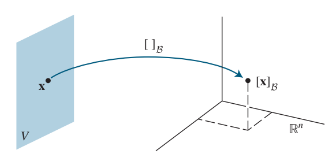
\includegraphics[width=8cm]{4_4_1}
  \end{center}

  \textbf{Theorem 4.9}\\
  Let $ \mathcal{B}=\{ b_1,...,b_n \} $ be a basis for a vector space $ V $. Then the coordinate mapping $ x \mapsto \begin{bmatrix}
    x
  \end{bmatrix}_\mathcal{B} $ is a one to one linear transformation from $ V $ onto $ \mathbb{R}^{n} $. 
  
  \textbf{Proof}\\
  Since linear transformations require that addition and scalar multiplication are preserved as they map vectors to other vectors that are within the span defined by the basis of $ V $. 

  Take two vectors in $ V $
  \[
    u=c_1b_1+...+c_nb_n \qquad w=d_1b_1+...+d_nb_n
  \]

  Then by using vector operations
  \[
    u+w=(c_1+d_1)b_1+...+(c_n+d_n)b_n
  \]

  It follows that
  \[
    \begin{bmatrix}
      u+w
    \end{bmatrix}_\mathcal{B}=\begin{bmatrix}
      c_1+d_1\\
      \vdots\\
      c_n+d_n
    \end{bmatrix}=\begin{bmatrix}
      c_1\\
      \vdots\\
      c_n
    \end{bmatrix}+
    \begin{bmatrix}
      d_1\\
      \vdots\\
      d_n
    \end{bmatrix}=
    \begin{bmatrix}
      u
    \end{bmatrix}_\mathcal{B}+
    \begin{bmatrix}
      w
    \end{bmatrix}_\mathcal{B}
  \]
  
  So the coordinate mapping preserves addition. Then if $ r $ is any scalar, then
  \[
    ru=r(c_1b_1+...+c_nb_n)=(rc_1)b_1+...+(rc_n)b_n
  \]

  So
  \[
    \begin{bmatrix}
      ru
    \end{bmatrix}_\mathcal{B}=
    \begin{bmatrix}
      rc_1\\
      \vdots\\
      rc_n
    \end{bmatrix}=
    r\begin{bmatrix}
      c_1\\
      \vdots\\
      c_n
    \end{bmatrix}=r\begin{bmatrix}
      x
    \end{bmatrix}_\mathcal{B}
  \]

   Transformations are only linear transformations if scalar multiplication and vector addition are preserved under the transformation. Since coordinate mappings are also transformations which preserve scalar multiplication and vector addition, then by that logic, coordinate mappings are linear transformations.

   \textbf{Ex 5}\\
   Let $ \mathcal{B} $ be the standard basis of the space $ \mathbb{P}_3 $ of polynomials; that is, let $ \mathcal{B}=\{ 1,t,t^{2},t^{3} \} $. A typical $ p $ of element $ \mathbb{P}_3 $ has the form
   \[
     p(t)=a_0+a_1t+a_2t^{2}+a_3t^{3}
   \]

   Since $ p $ is already displayed as a linear transformation of the standard basis vectors, then
   \[
     \begin{bmatrix}
       p
     \end{bmatrix}_\mathcal{B}=\begin{bmatrix}
       a_0\\
       a_1\\
       a_2\\
       a_3
     \end{bmatrix}
   \]

   Thus the coordinate mapping $ p \mapsto \begin{bmatrix}
     p
   \end{bmatrix}_\mathcal{B} $ is an isomorphism from $ \mathbb{P}_3 $ onto $ \mathbb{R}^{4} $. All vector space operations in $ \mathbb{P}_3 $ corrspond to operations in $ \mathbb{R}^{4} $. 
   
   \textbf{Ex 6}\\
   Use coordinate vectors to verify that the polynomials $ 1+2t^{2},4+t+5t^{2}, ~\&~ 3+2t $ are linearly dependent in $ \mathbb{P}_2 $

   The coordinate mapping from Ex $ 5 $ produces the coordinate vectors $ (1,0,2),(4,1,2), ~\&~ (3,2,0) $ respectively. These vectors can be written as the columns of a matrix $ A $. Then through row operations we can determine if the columns of the augmented matrix $ Ax=0 $  are linearly independent or not.
   \[
     \begin{gathered}
     Ax=0 = \begin{bmatrix}
       1 &4 &3 &0\\
       0 &1 &2 &0\\
       2 &5 &0 &0
     \end{bmatrix} \to 
     \begin{bmatrix}
       1 &4 &3 &0\\
       0 &1 &2 &0\\
       0 &0 &0 &0
     \end{bmatrix}
     \end{gathered}
   \]

   The columns of $ A $ are linearly dependent. So the corresponding polynomials are linearly dependent.

   \textbf{Ex 7}\\
   Let
   \[
     v_1=\begin{bmatrix}
       3\\
       6\\
       2
     \end{bmatrix}, \qquad v_2=
     \begin{bmatrix}
       -1\\
       0\\
       1
     \end{bmatrix}, \qquad x=
     \begin{bmatrix}
       3\\
       12\\
       7
     \end{bmatrix}, \qquad \mathcal{B}=\{ v_1,v_2 \}
   \]

   Then $ \mathcal{B} $ is a basis for $ H= $ Span $ \{ v_1,v_2 \} $. Determine if $ x $ is in $ H $, and if it is, find the coordinate vector of $ x $ relative to $ \mathcal{B} $.

   If $ x $ is in $ H $, then the following vector equation is consistent
   \[
     c_1\begin{bmatrix}
       3\\
       6\\
       2
     \end{bmatrix}+
     c_2\begin{bmatrix}
       -1\\
       0\\
       1
     \end{bmatrix}=
     \begin{bmatrix}
       3\\
       12\\
       7
     \end{bmatrix}
   \]

   If the scalars $ c_1 ~\&~ c_2 $ exist, then they are the $ \mathcal{B} $  coordinates of $ x $.
   \[
     \begin{gathered}
     \begin{bmatrix}
       3 &-1 &3\\
       6 &0 &12\\
       2 &1 &7
     \end{bmatrix} \to 
     \begin{bmatrix}
       1 &0 &2\\
       0 &1 &3\\
       0 &0 &0
     \end{bmatrix}\\
     ~\\
     c_1=2, \qquad c_2=3\\
     ~\\
     \boxed{
     \begin{bmatrix}
       x
     \end{bmatrix}_\mathcal{B}=
     \begin{bmatrix}
       2\\
       3
     \end{bmatrix}}
     \end{gathered}
   \]
   
\end{document}
